En este documento se detalla el trabajo realizado en torno al diseño, implementación y validación \gcnote{\sout{entiendo que estaras haciendo el diseño, implementacion, y validacion, cierto}} de un prototipo de \gcnote{\sout{prototipo? Para acotarlo mas.}} sistema de adquisición de datos para detectores de muones. Este sistema fue diseñado en base a indicaciones y requerimientos específicos del Centro Científico Tecnológico de Valparaíso (CCTVal) para aplicaciones de detección de particulas y muongrafía de terrenos mineros \gcnote{\sout{Incluir una breve frase sobre el origen y contexto de uso para el desarrollo. Por ejemplo: ''El sistema de adquisicion fue diseñado en base a indicaciones y requerimientos especificos del CERN/CCTval para ser usado en aplicaciones de .....''}}. El sistema fue implementado en una matriz de puertas lógicas programable en campo, o FPGA (por su sigla en inglés, Field-programable gate array) \gcnote{\sout{Introducir el acronimo la primera vez que se usa}} utilizando SystemVerilog. \gcnote{\sout{borre la frase, pero no es necesario poner \emph{hardware} en cursivas. Vas a usar demasiados terminos en ingles, asi que quedaria raro el texto. Deja los terminos en fuente normal, y despues se ve cuales vale la pena destacar.}}

El presente capítulo relata el contexto, las principales motivaciones que originan este proyecto de titulación, el planteamiento del problema, sus alcances y las contribuciones asociadas. Al final del capítulo se incluye además la organización del documento y detalles de cada capítulo.

\section{Contexto}
\gcnote{Articula mejor el texto para que fluya mejor. Estas usando frases cortas separadas por puntos seguidos, que lo hacen ver como un telegrama. Cada vez que termines un texto, leelo en voz alta siguiendo las reglas gramaticales del colegio, y eso te dara una idea de donde poner las puntuaciones. Si se lee muy golpeado o interrumpido es indicacion de que hay demasiados puntos, si te quedas sin aire en algun frase es indicacion de que falta una coma o la frase esta muy larga, etc.}

	El planeta tierra es constantemente bombardeado por rayos cósmicos, los cuales provienen del espacio exterior y corresponden principalmente a partículas cargadas, como protones y núcleos atómicos. \gcnote{\sout{que es lo que se caracteriza por viajar a grandes velocidades? Esto gramaticalmente se llama un \emph{dangling modifier}. Estudia en que consiste y evitalos en el resto del documento y para el resto de tu vida. Tambien tiene que ver con el exceso de puntuacion.}} El origen de estos rayos es variado, y aunque la fuente de algunos de estos rayos es desconocida, la mayor parte de ellos proviene de tormentas solares, agujeros negros e incluso eventos astronómicos asociados al origen del universo. La velocidad alcanzada por estas partículas cósmicas es tan grande, que entran en la categoría de partículas de altas energías, alcanzando desde unos cuantos GeV (Giga Electron Volts) para partículas provenientes del sol, hasta más de 1000 TeV para rayos originados en centros galácticos y agujeros negros. \gcnote{\sout{Falta tambien un contexto de donde provienen o algo asi (no aparecen de la nada) y por que son relevantes, aunque sea algo intuitivo para el lector comun y corriente.}}
	
	El estudio de los rayos cósmicos permite conocer detalles sobre eventos astronómicos lejanos, pero también da la oportunidad de dilucidar características propias de la materia atravesada por estas partículas.
	
	Los rayos cósmicos inciden en el planeta tierra e interactúan con la atmósfera terrestre, produciendo la ionización del medio y decayendo en partículas secundarias. Estas últimas vuelven a interactuar con otras partículas, generando una efecto en cadena y produciendo así una lluvia de rayos subatómicos sobre la corteza terrestre. La figura \ref{img:cosmic-ray} corresponde a una representación artística de la lluvia de partículas originada por radiación cósmica.
	
	Cerca del 70\% de las partículas que logran llegar a la superficie del planeta corresponden a muones. \gcnote{dangling modifier}Estos poseen la misma carga que un electrón, pero con una masa cerca de 200 veces mayor. \gcnote{dangling modifier}Esta característica, sumada a su altísima velocidad \gcnote{cuanto?}, permite que los muones pasen a través de la materia. \gcnote{dangling modifier. El ultimo que marco. Corregir en todo el documento.}Incluso, son capaces de alcanzar zonas bajo tierra durante el transcurso de su vida media, correspondiente a aproximadamente $2\mu s$.
	
	Al atravesar materia, los muones son absorbidos o su energía se ve disminuida. Detectarlos y medir su energía permite entonces conocer propiedades de la materia que ha sido atravesada por estas partículas. Por ejemplo, es posible realizar un mapa de densidad de terreno a partir de los cruces de muones, proceso conocido como muongrafía o tomografía muónica \gcnote{seria bueno ir dando referencias de literatura para estos conceptos, en caso de que el lector quiera saber mas al respecto. Dar tambien un ejemplo de aplicaciones practicas (mineria, topografia, otros.). Esto es en forma breve, y despues en el resto del capitulo explicas mas detalles de las aplicaciones especificas. COnsidera la motivacion como un trailer motivacional para que el lector quiera seguir viendo la pelicula. Detectar muones es aburrido, las aplicaciones que tiene este tipo de tecnologia en entornos productivos es lo interesante desde el punto de vista de ingenieria.}.
	
	Para llevar a cabo mediciones y análisis de detección de muones se requieren detectores, interfaces de lectura, análisis computacional, y por supuesto, un sistema de adquisición de datos capaz de  transformar las características físicas de eventos detectados a datos computables y analizables para extracción e interpretación de la información.
	
	\begin{figure}[h]
		\centering
		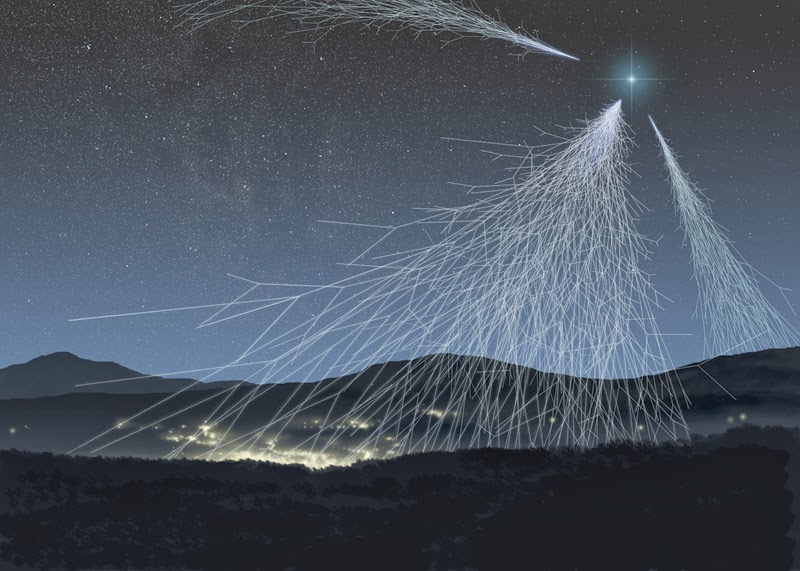
\includegraphics[scale=0.4]{cosmic_rays.jpg}
		\caption{Representación artística de rayos cósmicos y lluvia de partículas subatómicas sobre la corteza terrestre.}
		\label{img:cosmic-ray}
	\end{figure}
	
	
\section{Motivación}
	El ``Sistema de adquisición de datos para detectores de muones'' nace como un requerimiento del Centro Científico Tecnológico de Valparaíso (CCTVal) para aplicaciones de física de partículas, en el marco del proyecto ``sTGC Minería''. 
	
	Uno de los objetivos principales de ``sTGC Minería'' es realizar tomografías muónicas de terreno minero detectando partículas que provengan de radiación cósmica, método similar al que se utiliza para encontrar criptas y cavernas en pirámides egipcias\gcnote{interesante, pero da una referencia a algun articulo}. Estas tomografías sientan las bases para la detección de cavernas subterráneas y estimación de densidad en terrenos mineros. La figura \ref{img:muongrafia} corresponde a una muongrafía de un corte trasversal de terreno. \gcnote{explicar un poco mejor la figura. Que informacion util entrega esa figura? Que significa el mapa de colores?}

	
	Producto de la colaboración existente entre CCTVal y el experimento ATLAS, en CERN, el centro cuenta con las herramientas y conocimientos necesarios para la fabricación de detectores de muones en Chile. Los detectores de partículas a utilizar en ``sTGC Minería'' corresponden precisamente a unos basados en los detectores del espectrómetro de muones presente en el experimento ATLAS.
	
	\begin{figure}[h]
		\centering
		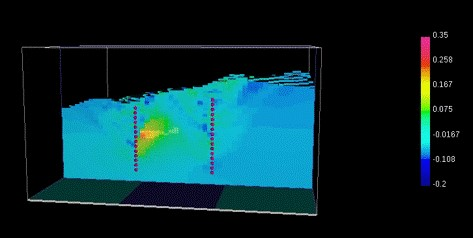
\includegraphics[scale=1]{Stgcgif.jpg}
		\caption{Imagen referencial de un mapa de calor para representación de densidades en un corte transversal de terreno.}
		\label{img:muongrafia}
	\end{figure}
	

\section{Planteamiento del Problema}
\label{sec:planteamiento}
	La detección de muones implica una serie de etapas y detectores desarrollados con tecnologías que se utilizan en experimentos tales como ATLAS, en CERN \gcnote{Introducir los acronimos}. Particularmente en ``sTGC Minería'', se requiere un sistema que sea capaz de captar las señales generadas por los detectores y que determine de manera fiable y precisa \gcnote{a que te refieres con fiable y precisa?} aquellas zonas del detector por las cuales ha pasado un muon.
	
	El ``Sistema de adquisición de datos para detectores de muones'' cumplirá con las funciones de adquirir, discriminar y estructurar la información captada desde el detector, para así contribuir a la tomografía muónica del terreno.
	
 	Como objetivo principal se tiene el detectar la posición del paso de muones en un detector de configuración matricial, indicando el o los cuadrantes \gcnote{no se han explicado lo de los cuadrantes ni cosa asociadas. Quizas debas mover las especificaciones tecnicas generales antes.} que han sido excitados por el paso de las partículas, de manera fiable y eficiente \gcnote{antes dijiste eficiente y precisa. Se consistente con el lenguaje tecnico, no es un reporte literario ni de poesia (lo cual no quiere decir que puede estar mal escrito).}, logrando captar gran \gcnote{cuantas? Evita el uso/abuso de terminos no cuantificables y subjetivos. Da al menos ordenes (decenas, cientos, miles?)}{cantidad de señales íntegramente \gcnote{que es integramente? que no sean corruptas o eticamente correctas?}.
 	
 	La figura \ref{img:sistema} ilustra el sistema de muongrafía de terreno considerando un solo detector de muones. Para su operación, utiliza dos detectores centelleantes secundarios, un sistema de coincidencias y una interfaz de lectura. El sistema de adquisición de datos capta y discrimina los pulsos generados según se correspondan con la señal de coincidencia asociada a los detectores centelleantes. La información resultante es comunicada a etapas posteriores para análisis de datos. \gcnote{Esto deberia ir antes. Ver comentarios anteriores.}
	
	Es requisito del proyecto que este sistema sea concebido como una herramienta adaptada para operar con detectores de mayor tamaño o con arreglos de detectores individuales, permitiendo el análisis de zonas de mayor área o el estudio de trayectorias de partículas con detectores superpuestos. Esto implica que el sistema debe ser de naturaleza modular y expansible, sobre todo en torno a la cantidad de señales que es capaz de procesar.  \gcnote{No queda claro que es lo que ya esta hecho y que es lo que haras tu? Estas haciendo el detector completo, o solo el sistema de adquisicion? Explicar mejor. Tambien dejar claro que es un prototipo de cierto tamaño.}
	
	Como objetivo secundario, el proyecto debe ser una herramienta replicable que esté disponible para ser utilizada en nuevos proyectos y experimentos del centro de investigación. Así mismo, el desarrollo y la documentación del proceso debe ser un aporte al conocimiento sobre la implementación de sistemas electrónicos para la detección y análisis de partículas utilizando estas tecnologías, ya que es uno de los primeros en ser desarrollados y probados por el centro. \gcnote{Esto ultimo deberia plantearse como una motivacion. ''Actualmente no se tiene conocimiento sobre esto, por lo que en este proyecto se busca adquirir experiencia practica...''}
	
	\begin{figure}[h]
		\centering
		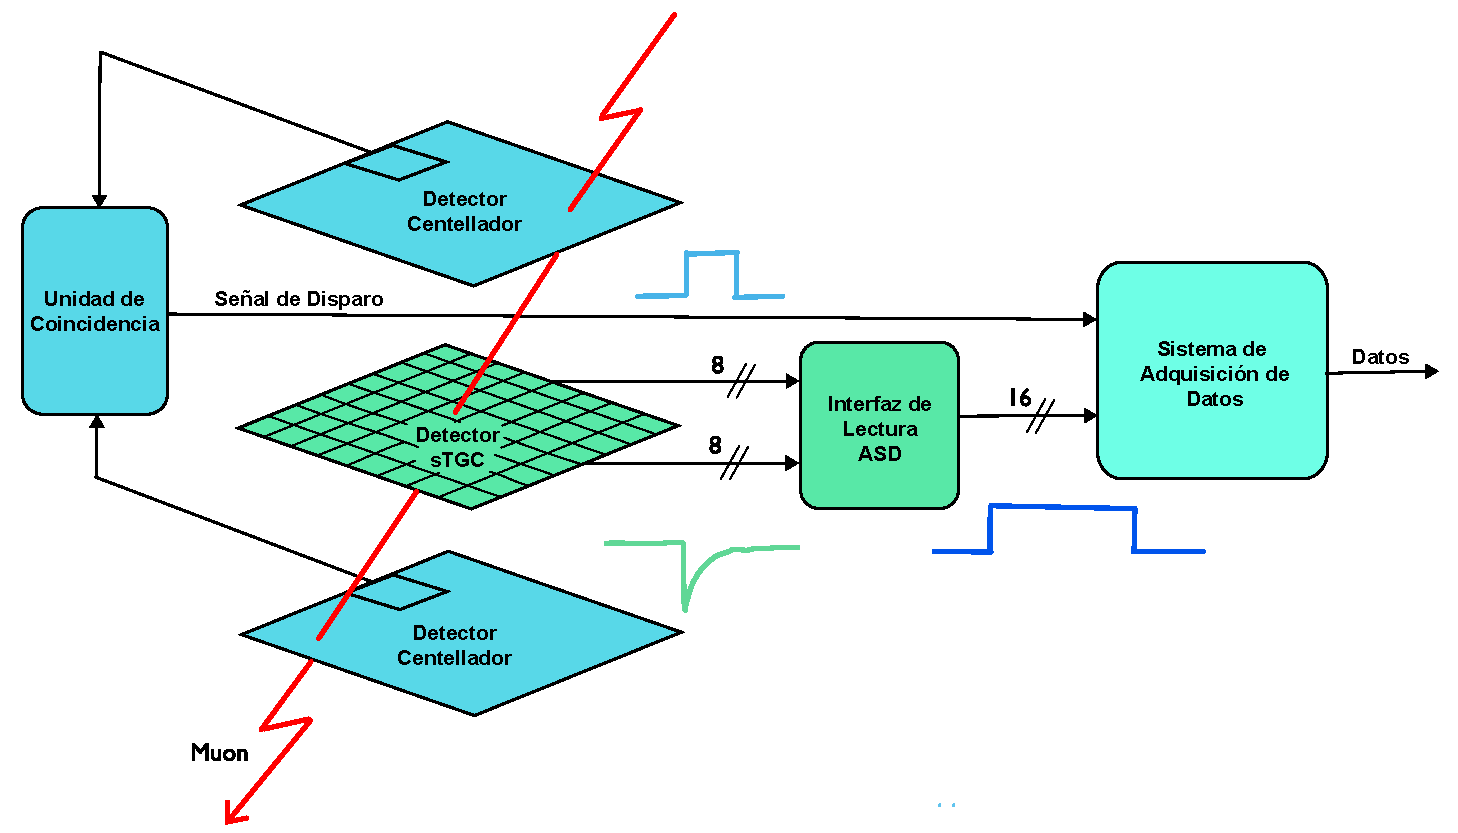
\includegraphics[scale=0.55]{sistema.pdf}
		\caption{Diagrama del sistema de muongrafía de terreno para un solo detector. Se incluyen en azul las formas de señal asociadas a la señal de disparo, eventos de detección, y lectura de pulsos.}
		\label{img:sistema}
	\end{figure}						

\section{Alcances y contribuciones}

\gcnote{Toda esta seccion debe ser mas concreta y especifica.}
	Se espera que este sistema sea capaz de generar información suficiente para representar la ubicación del paso de las partículas en la superficie del detector, determinando cuadrantes de $1cm^2$ que hayan sido excitados por el cruce de partículas.
	
	El sistema deberá ser capaz de captar cantidades pares arbitrarias de canales, discriminando partículas mediante la utilización de las señales de disparo disponibles.
	
	La información generada pasará a etapas siguientes de análisis detallado o de representación gráfica, por lo cual es importante que el sistema sea capaz de entregar información pertinentemente ordenada, procesada y seleccionada para dichos fines.
	
	Finalmente, uno de los principales aportes recae en la documentación respecto a entorno, operación y desarrollo del sistema en cuestión. Esto con el fin de facilitar la implementación del diseño en nuevos sistemas, permitir profundizar y mejorar la propuesta diseñada y entregar las herramientas al centro y a futuros estudiantes para operar dispositivos que posean etapas equivalentes.


\section{Organización del documento.}

	Este documento se estructura de la siguiente manera: \gcnote{demasiados capitulos. No deberian ser mas de 5 o 6.}
	
	\begin{itemize}
		\item El \textbf{Capítulo \ref{cap:art}} incluye el estado del arte en cuanto a dispositivos de adquisición de datos para partículas de altas energías.
		\item El \textbf{Capítulo \ref{cap:arq}} detalla la arquitectura propuesta para la realización de este proyecto, contemplando componentes y estructura del mismo.
		\item El \textbf{Capítulo \ref{cap:stgc}} describe las características del detector de partículas utilizado.
		\item El \textbf{Capítulo \ref{cap:asd}} resume las especificaciones del sistema de lectura para señales provenientes del detector, además de explicar su estructura y funcionamiento.
		\item El \textbf{Capítulo \ref{cap:sampling}} detalla la primera etapa de diseño de hardware, encargada de tomar muestras de los pulsos digitales provenientes de la etapa inmediatamente anterior.
		\item El \textbf{Capitulo \ref{cap:discriminator}} trata sobre el diseño para la etapa de discriminación del sistema de adquisición, la cual selecciona aquellos eventos temporalmente coincidentes con una señal de disparo.
		\item El \textbf{Capítulo \ref{cap:structure}} describe la etapa de estructuración de eventos y su diseño, en donde la información de pulsos capturados es asociada los canales y cuadrantes correspondientes.
		\item El \textbf{Capítulo \ref{cap:analysis}} detalla la etapa de análisis de datos para determinación del paso de partículas cargadas por el detector.
		\item El \textbf{Capítulo \ref{cap:sync}} trata sobre la etapa de sincronización y su diseño, en donde se coordinan eventos capturados por distintos detectores simultáneamente.
		\item El \textbf{Capítulo \ref{cap:comm}} se refiere a la etapa de comunicación serial, a través de la cual el sistema se comunica con computadores externos para envío de datos.
		\item El \textbf{Capítulo \ref{cap:test}} incluye pruebas realizadas en el sistema con el fin de comprobar funcionamiento y resultados del dispositivo.
		\item El \textbf{Capítulo \ref{cap:insights}} resume los resultados de experimentación y desempeño del sistema diseñado.
		\item El \textbf{Capítulo \ref{cap:conclusiones}} incluye las conclusiones finales y trabajo futuro propuesto a partir de lo realizado en este proyecto de titulación.
	\end{itemize}

